\documentclass[aspectratio=169,9pt]{beamer}
\usepackage[T5]{fontenc}
\usepackage[utf8]{inputenc}
\usepackage[vietnamese]{babel}
\usepackage{lmodern}
\usepackage{graphicx}
\usepackage{booktabs}
\usepackage{tabularx}
\usepackage{array}
\usepackage{ragged2e}
\usepackage{tikz}
\usepackage{tcolorbox}
\usetikzlibrary{arrows.meta,calc,positioning,shapes.geometric}
\graphicspath{{images/}}

\definecolor{CoboRed}{RGB}{172,29,33}
\definecolor{CoboBlue}{RGB}{31,100,157}
\definecolor{CoboGreen}{RGB}{31,132,79}
\definecolor{CoboText}{RGB}{42,44,52}
\definecolor{CoboGray}{RGB}{116,122,134}
\definecolor{CoboLight}{RGB}{246,247,249}
\definecolor{CoboLine}{RGB}{143,151,164}

\setbeamertemplate{navigation symbols}{}
\setbeamertemplate{headline}{}
\setbeamersize{text margin left=0.48cm,text margin right=0.48cm}
\setbeamercolor{normal text}{fg=CoboText,bg=white}
\setbeamercolor{frametitle}{fg=white,bg=CoboRed}
\setbeamerfont{normal text}{size=\fontsize{8.8}{10.6}\selectfont}
\setbeamerfont{frametitle}{size=\fontsize{12.3}{14.2}\selectfont,series=\bfseries}
\setbeamerfont{itemize/enumerate body}{size=\fontsize{8.8}{10.6}\selectfont}
\setbeamercolor{itemize item}{fg=CoboRed}
\setbeamercolor{itemize subitem}{fg=CoboRed}
\setbeamertemplate{itemize item}{\raisebox{0.12ex}{\scriptsize$\blacktriangleright$}}
\setbeamertemplate{itemize subitem}{\raisebox{0.12ex}{\tiny$\blacktriangleright$}}
\setbeamertemplate{enumerate item}{\color{CoboRed}\insertenumlabel.}

\setbeamertemplate{frametitle}{
  \nointerlineskip
  \begin{beamercolorbox}[wd=\paperwidth,ht=0.67cm,dp=0.36cm,center]{frametitle}
    \insertframetitle
  \end{beamercolorbox}
}
\setbeamertemplate{footline}{
  \leavevmode
  \hbox to \paperwidth{\hfill
    \colorbox{CoboRed}{\makebox[0.29cm][c]{\color{white}\fontsize{5.2}{5.2}\selectfont\insertframenumber}}
    \hspace{0.46cm}}
  \vspace{0.28cm}
}

\newcommand{\source}[1]{\vfill{\color{CoboGray}\fontsize{5.4}{6.4}\selectfont\itshape Nguồn: #1.\par}}
\newcommand{\captiontext}[1]{{\fontsize{6.2}{7.2}\selectfont #1\par}}
\newcommand{\smallnote}[1]{{\fontsize{7.1}{8.5}\selectfont #1\par}}
\newcommand{\redlabel}[1]{\colorbox{CoboRed}{\makebox[0.46cm][c]{\color{white}\bfseries #1}}}
\newcommand{\tagbox}[2]{\colorbox{#1}{\strut\hspace{0.14cm}\color{white}\bfseries\fontsize{6.8}{8}\selectfont #2\hspace{0.14cm}}}
\newcommand{\heading}[1]{{\bfseries #1\par}}
\newcommand{\tightitems}{\setlength{\itemsep}{0.12em}\setlength{\parskip}{0pt}\setlength{\parsep}{0pt}}

\tcbset{
  cobobox/.style={colback=white,colframe=CoboLine,boxrule=0.45pt,arc=1.2mm,left=1.5mm,right=1.5mm,top=1mm,bottom=1mm,before skip=0pt,after skip=0pt},
  redbox/.style={colback=CoboLight,colframe=CoboLine,boxrule=0.4pt,arc=0mm,left=1.2mm,right=1.2mm,top=0mm,bottom=1mm,fonttitle=\bfseries,coltitle=white,colbacktitle=CoboRed,titlerule=0pt}
}
\newcolumntype{L}[1]{>{\RaggedRight\arraybackslash}p{#1}}
\newcolumntype{R}[1]{>{\RaggedLeft\arraybackslash}p{#1}}
\newcolumntype{C}[1]{>{\Centering\arraybackslash}p{#1}}

\begin{document}

\begin{frame}
  \centering
  \vspace{-0.22cm}
  {\fontsize{10.2}{12}\selectfont Báo cáo đọc bài báo\par}
  \vspace{0.55cm}
  {\color{CoboRed}\bfseries\fontsize{12.2}{14.5}\selectfont
    HỌC VIỆN CÔNG NGHỆ BƯU CHÍNH VIỄN THÔNG\par}
  \vspace{0.07cm}
  {\bfseries\fontsize{8.7}{10.2}\selectfont Khoa Kĩ thuật Điện tử 1\par}
  \vspace{0.35cm}
  {\color{CoboRed}\rule{0.59\paperwidth}{0.45pt}\par}
  \vspace{0.25cm}
  {\color{CoboRed}\bfseries\fontsize{11.2}{12.2}\selectfont
    COBOGESTURE: A CONTINUOUS HAND GESTURE DATASET\par
    AND RECOGNITION METHOD FOR HUMAN-COLLABORATIVE ROBOT\par
    INTERACTION\par}
  \vspace{0.18cm}
  {\bfseries\fontsize{8.6}{10}\selectfont Phuong-Dung Nguyen et al., IEEE Access, 2026\par}
  {\fontsize{7.8}{9}\selectfont DOI: 10.1109/ACCESS.2026.3664027\par}
  \vspace{0.35cm}
  \tagbox{CoboRed}{Hand Gesture Recognition}\hspace{0.16cm}
  \tagbox{CoboBlue}{Human-Cobot Interaction}\hspace{0.16cm}
  \tagbox{CoboGreen}{Edge Device}
\end{frame}

\begin{frame}{Nội dung trình bày}
  \vspace{0.30cm}
  \begin{tabular}{@{}c@{\hspace{0.25cm}}L{3.35cm}L{8.40cm}@{}}
    \redlabel{1} & \textcolor{CoboRed}{\bfseries Bối cảnh và bài toán} & Nhận dạng cử chỉ tay trong tương tác người--robot cộng tác.\\[0.34cm]
    \redlabel{2} & \textcolor{CoboRed}{\bfseries Dataset CoboGesture} & Quy trình thu thập, đặc điểm dữ liệu và ý nghĩa.\\[0.34cm]
    \redlabel{3} & \textcolor{CoboRed}{\bfseries Phương pháp đề xuất} & VideoMAE, RGB-CoGes và SkeRGB-CoGes.\\[0.34cm]
    \redlabel{4} & \textcolor{CoboRed}{\bfseries Kết quả thực nghiệm} & Isolated recognition, continuous recognition và triển khai edge.\\[0.34cm]
    \redlabel{5} & \textcolor{CoboRed}{\bfseries Đánh giá tổng hợp} & Đóng góp, hạn chế và hướng phát triển.
  \end{tabular}
\end{frame}

\begin{frame}{1. Bối cảnh nghiên cứu}
  \vspace{0.04cm}
  \begin{columns}[T,onlytextwidth]
    \begin{column}{0.62\textwidth}
      \heading{Robot cộng tác trong môi trường công nghiệp}
      \begin{itemize}\tightitems
        \item Cobot được thiết kế để làm việc gần con người trong cùng không gian.
        \item Giao tiếp người--robot cần tự nhiên, nhanh và dễ học với người vận hành.
        \item Cử chỉ tay là kênh giao tiếp trực quan, ít phụ thuộc ngôn ngữ và không cần thiết bị đeo.
      \end{itemize}
      \vspace{0.16cm}
      \begin{tcolorbox}[cobobox]
        \textbf{Mục tiêu ứng dụng:} người vận hành dùng cử chỉ để ra lệnh bắt đầu, dừng, xác nhận, hủy thao tác hoặc điều hướng robot.
      \end{tcolorbox}
    \end{column}
    \begin{column}{0.34\textwidth}
      \centering
      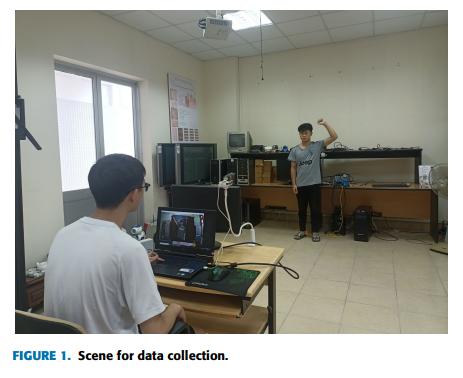
\includegraphics[width=0.88\linewidth]{image-4.png}\par
      \vspace{0.12cm}
      \captiontext{Bối cảnh thu thập dữ liệu trong phòng thí nghiệm.}
    \end{column}
  \end{columns}
  \source{Nguyen et al., IEEE Access, 2026}
\end{frame}

\begin{frame}{2. Bài toán nghiên cứu}
  \vspace{0.15cm}
  \centering
  \begin{tikzpicture}[node distance=0.75cm,>=Stealth]
    \tikzset{stage/.style={draw=CoboRed!65,rounded corners=1.2mm,fill=CoboLight,minimum width=2.25cm,minimum height=0.82cm,align=center,font=\fontsize{7.5}{8.8}\selectfont}}
    \node[stage] (a) {Camera RGB\\video liên tục};
    \node[stage,right=of a] (b) {Phát hiện đoạn\\có cử chỉ};
    \node[stage,right=of b] (c) {Phân loại\\cử chỉ};
    \node[stage,right=of c] (d) {Lệnh điều khiển\\cobot};
    \draw[->,CoboRed,thin] (a) -- (b);
    \draw[->,CoboRed,thin] (b) -- (c);
    \draw[->,CoboRed,thin] (c) -- (d);
  \end{tikzpicture}
  \vspace{0.45cm}
  \begin{columns}[T,onlytextwidth]
    \begin{column}{0.49\textwidth}
      \begin{tcolorbox}[redbox,title=Đầu vào]
        Video dài, chưa cắt sẵn, gồm nhiều cử chỉ và các khoảng không có cử chỉ điều khiển.
      \end{tcolorbox}
    \end{column}
    \begin{column}{0.49\textwidth}
      \begin{tcolorbox}[redbox,title=Đầu ra]
        Nhãn cử chỉ theo thời gian: lớp cử chỉ, thời điểm bắt đầu và thời điểm kết thúc.
      \end{tcolorbox}
    \end{column}
  \end{columns}
  \vspace{0.34cm}
  \begin{tcolorbox}[cobobox]
    Bài toán thuộc nhóm \textbf{continuous hand gesture recognition}, gần với điều kiện triển khai thực tế hơn so với nhận dạng trên video đã cắt.
  \end{tcolorbox}
\end{frame}

\begin{frame}{3. Hạn chế của các nghiên cứu trước}
  \vspace{0.16cm}
  \begin{columns}[T,onlytextwidth]
    \begin{column}{0.315\textwidth}
      \begin{tcolorbox}[cobobox,height=2.42cm]
        \heading{Dữ liệu}
        Nhiều dataset không chuyên biệt cho điều khiển cobot; bối cảnh và bộ cử chỉ không khớp môi trường công nghiệp.
      \end{tcolorbox}
    \end{column}
    \begin{column}{0.315\textwidth}
      \begin{tcolorbox}[cobobox,height=2.42cm]
        \heading{Bài toán}
        Phần lớn phương pháp tập trung vào isolated recognition: mỗi video đã chứa đúng một cử chỉ.
      \end{tcolorbox}
    \end{column}
    \begin{column}{0.315\textwidth}
      \begin{tcolorbox}[cobobox,height=2.42cm]
        \heading{Triển khai}
        Ít công trình đánh giá tốc độ, độ trễ và khả năng chạy trên thiết bị biên.
      \end{tcolorbox}
    \end{column}
  \end{columns}
  \vspace{0.38cm}
  \centering
  \begin{tikzpicture}[>=Stealth]
    \tikzset{reality/.style={draw=CoboLine,rounded corners=1mm,minimum width=2.85cm,minimum height=0.65cm,align=center,font=\fontsize{7}{8}\selectfont}}
    \node[reality,fill=CoboRed!6] (a) at (0,0) {Video đã cắt sẵn};
    \node[reality,fill=CoboBlue!5] (b) at (4.0,0) {Video liên tục};
    \node[reality,fill=CoboGreen!7] (c) at (7.3,0) {Thiết bị edge};
    \draw[->,CoboText] (-1.4,-0.62) -- (9.0,-0.62) node[right,font=\fontsize{6.8}{8}\selectfont]{Mức độ gần thực tế};
  \end{tikzpicture}
  \source{Tổng hợp từ phần Introduction và Related Work của bài báo}
\end{frame}

\begin{frame}{4. Đóng góp chính của bài báo}
  \vspace{0.05cm}
  \begin{columns}[T,onlytextwidth]
    \begin{column}{0.62\textwidth}
      \begin{enumerate}\tightitems
        \item Xây dựng dataset \textbf{CoboGesture} cho continuous hand gesture recognition trong human-cobot interaction.
        \item Đề xuất hai pipeline nhận dạng liên tục: \textbf{RGB-CoGes} và \textbf{SkeRGB-CoGes}.
        \item Sử dụng \textbf{VideoMAE/VideoMAEv2} để học đặc trưng không gian--thời gian từ video RGB.
        \item Đánh giá trên cả offline benchmark và triển khai online trên edge device.
      \end{enumerate}
    \end{column}
    \begin{column}{0.34\textwidth}
      \heading{Tóm tắt đóng góp}
      \begin{itemize}\tightitems
        \item Dataset: CoboGesture, 19 gestures + No-gesture.
        \item Method: RGB-CoGes và SkeRGB-CoGes.
        \item Backbone: VideoMAE/VideoMAEv2.
        \item Deployment: Jetson AGX Orin.
      \end{itemize}
    \end{column}
  \end{columns}
\end{frame}

\begin{frame}{5. Dataset CoboGesture}
  \vspace{0.02cm}
  \begin{columns}[T,onlytextwidth]
    \begin{column}{0.59\textwidth}
      \heading{Đặc điểm chính}
      \begin{itemize}\tightitems
        \item Bộ dữ liệu video RGB cho nhận dạng cử chỉ tay liên tục.
        \item Gồm \textbf{19 cử chỉ} phục vụ tương tác người--cobot.
        \item Có thêm lớp \textbf{No-gesture} cho các đoạn không phải lệnh điều khiển.
        \item Mỗi video chứa chuỗi nhiều cử chỉ, được gán nhãn theo thời gian.
      \end{itemize}
      \vspace{0.20cm}
      \begin{tcolorbox}[cobobox]
        Điểm quan trọng của dataset là nhãn không chỉ cho biết \textbf{cử chỉ gì}, mà còn cho biết \textbf{khi nào bắt đầu} và \textbf{khi nào kết thúc}.
      \end{tcolorbox}
    \end{column}
    \begin{column}{0.37\textwidth}
      \centering
      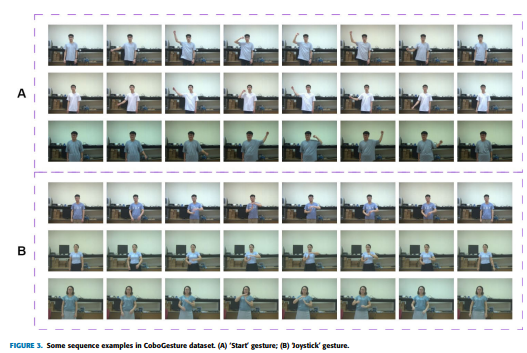
\includegraphics[width=\linewidth]{image-7.png}\par
      \vspace{0.15cm}
      \captiontext{Ví dụ chuỗi cử chỉ trong CoboGesture.}
    \end{column}
  \end{columns}
\end{frame}

\begin{frame}{6. Quy trình thu thập dữ liệu}
  \vspace{0.05cm}
  \begin{columns}[T,onlytextwidth]
    \begin{column}{0.50\textwidth}
      \centering
      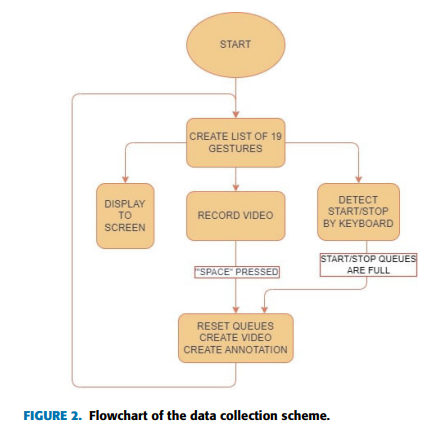
\includegraphics[height=4.15cm]{image-5.png}
    \end{column}
    \begin{column}{0.46\textwidth}
      \heading{Thiết lập thu thập}
      \begin{itemize}\tightitems
        \item Camera công nghiệp FLIR RGB, độ phân giải \textbf{1440$\times$1080}, tốc độ \textbf{30 FPS}.
        \item Camera đặt cách người thực hiện khoảng \textbf{2.5 m}, cao \textbf{1.1--1.2 m}.
        \item Người tham gia thực hiện cử chỉ theo hướng dẫn trên màn hình.
        \item Annotator đánh dấu thời điểm bắt đầu/kết thúc bằng bàn phím.
        \item Annotation được rà soát thủ công sau khi thu thập.
      \end{itemize}
    \end{column}
  \end{columns}
  \source{Figure 2 và phần Data Collection trong bài báo}
\end{frame}

\begin{frame}{7. Thống kê CoboGesture}
  \vspace{0.28cm}
  \begin{columns}[T,onlytextwidth]
    \begin{column}{0.42\textwidth}
      \centering
      \begin{tabular}{@{}L{3.00cm}R{2.30cm}@{}}
        \toprule
        \textbf{Người tham gia} & 50\\
        \textbf{Nữ / Nam} & 11 / 39\\
        \textbf{Video liên tục} & 150\\
        \textbf{Độ dài mỗi video} & 100--140 s\\
        \textbf{Mẫu cử chỉ} & 2,479\\
        \textbf{Số frame RGB} & 490,000\\
        \textbf{Tổng thời lượng} & \mbox{khoảng 4.5 giờ}\\
        \textbf{Số lớp cử chỉ} & \mbox{19 + No-gesture}\\
        \bottomrule
      \end{tabular}
    \end{column}
    \begin{column}{0.54\textwidth}
      \centering
      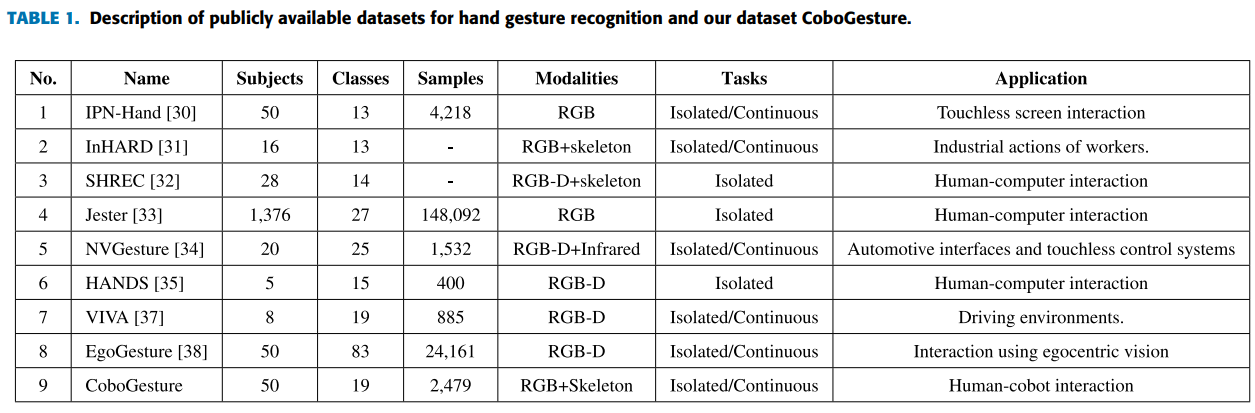
\includegraphics[width=\linewidth]{image.png}\par
      \vspace{0.20cm}
      \captiontext{Thống kê số mẫu và thời lượng trung bình theo lớp.}
    \end{column}
  \end{columns}
  \source{Nguyen et al., IEEE Access, 2026}
\end{frame}

\begin{frame}{8. Isolated và continuous recognition}
  \vspace{0.02cm}
  \centering
  {\fontsize{7.7}{9.2}\selectfont
  \renewcommand{\arraystretch}{1.20}
  \begin{tabular}{@{}L{2.45cm}L{4.18cm}L{4.25cm}@{}}
    \toprule
    \textbf{Tiêu chí} & \textbf{Isolated recognition} & \textbf{Continuous recognition}\\
    \midrule
    Đầu vào & Video ngắn đã cắt sẵn & Video dài, chưa cắt sẵn\\
    Số cử chỉ & Thường một cử chỉ & Nhiều cử chỉ và khoảng No-gesture\\
    Nhiệm vụ & Phân loại cử chỉ & Phát hiện đoạn cử chỉ và phân loại\\
    Đầu ra & Một nhãn cho video & Nhãn theo thời gian/frame\\
    Metric chính & Accuracy & Frame-wise Accuracy, Overlap Score\\
    Mức độ ứng dụng & Giai đoạn huấn luyện/benchmark & Gần với hệ thống vận hành thực tế\\
    \bottomrule
  \end{tabular}}
  \vspace{0.32cm}
  \begin{tcolorbox}[cobobox]
    Trong bài báo, mô hình được huấn luyện từ các đoạn isolated, sau đó được sử dụng trong pipeline continuous recognition.
  \end{tcolorbox}
\end{frame}

\begin{frame}{9. Pipeline tổng quát}
  \centering
  \vspace{-0.03cm}
  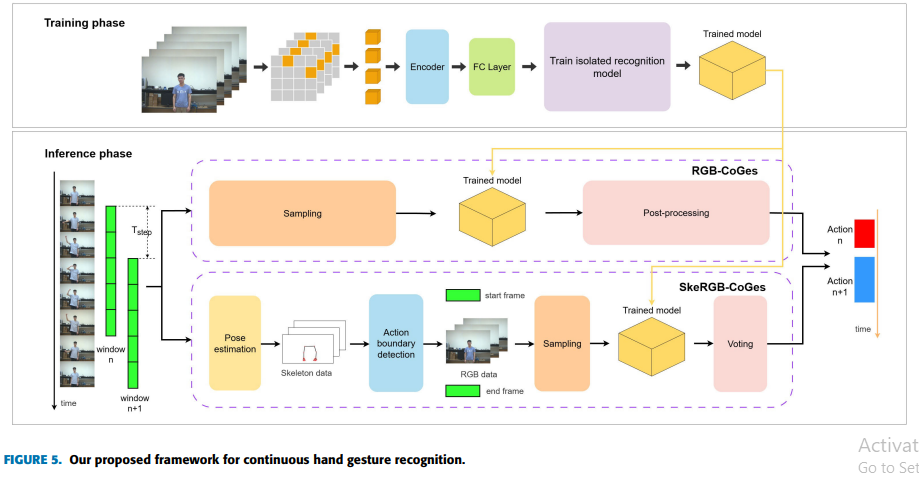
\includegraphics[width=0.48\linewidth]{image-1.png}
  \vspace{0.18cm}
  \begin{itemize}\tightitems
    \item \textbf{Training phase:} cắt video thành isolated gesture, huấn luyện VideoMAE/VideoMAEv2 để phân loại.
    \item \textbf{Inference phase:} áp dụng mô hình đã huấn luyện lên video liên tục bằng RGB-CoGes hoặc SkeRGB-CoGes.
    \item \textbf{Post-processing:} voting/làm mượt nhãn để giảm nhiễu dự đoán theo thời gian.
  \end{itemize}
\end{frame}

\begin{frame}{10. Mô hình nền VideoMAE/VideoMAEv2}
  \vspace{0.07cm}
  \begin{columns}[T,onlytextwidth]
    \begin{column}{0.60\textwidth}
      \heading{Vai trò trong bài báo}
      \begin{itemize}\tightitems
        \item Học đặc trưng không gian--thời gian từ chuỗi ảnh RGB.
        \item Tận dụng mô hình đã pretrain trên tập dữ liệu video lớn.
        \item Fine-tune cho bài toán phân loại 19 cử chỉ trong CoboGesture.
        \item Decoder của masked autoencoder được thay bằng classification head.
      \end{itemize}
      \source{VideoMAE: masked autoencoder cho video representation learning}
    \end{column}
    \begin{column}{0.34\textwidth}
      \centering
      \begin{tikzpicture}[node distance=0.18cm,>=Stealth]
        \tikzset{model/.style={draw=CoboRed!65,rounded corners=1mm,fill=CoboLight,minimum width=2.65cm,minimum height=0.52cm,align=center,font=\fontsize{6.4}{7.4}\selectfont}}
        \node[model] (a) {Video clip};
        \node[model,below=of a] (b) {Chia thành patch/tube};
        \node[model,below=of b] (c) {Che một phần dữ liệu};
        \node[model,below=of c] (d) {ViT encoder học biểu diễn};
        \node[model,below=of d] (e) {Classifier head};
        \node[model,below=of e] (f) {Nhãn cử chỉ};
        \foreach \x/\y in {a/b,b/c,c/d,d/e,e/f}{\draw[->,CoboRed] (\x) -- (\y);}
      \end{tikzpicture}
    \end{column}
  \end{columns}
\end{frame}

\begin{frame}{11. Phương pháp RGB-CoGes}
  \vspace{0.10cm}
  \begin{columns}[T,onlytextwidth]
    \begin{column}{0.57\textwidth}
      \centering
      \begin{tikzpicture}[>=Stealth]
        \tikzset{win/.style={draw=CoboBlue,rounded corners=1mm,minimum width=1.50cm,minimum height=0.48cm},classifier/.style={draw=CoboRed!70,rounded corners=1mm,fill=CoboLight,minimum width=3.15cm,minimum height=0.62cm,align=center,font=\fontsize{6.8}{8}\selectfont}}
        \foreach \i in {0,...,9}{\draw[CoboLine] (0.34*\i,0) rectangle +(0.29,0.45);}
        \draw[CoboRed,rounded corners=1mm] (0.30,-0.05) rectangle +(1.52,0.55);
        \draw[CoboBlue,rounded corners=1mm] (1.05,-0.05) rectangle +(1.52,0.55);
        \draw[CoboGreen,rounded corners=1mm] (1.80,-0.05) rectangle +(1.52,0.55);
        \node[classifier] (clf) at (1.75,1.08) {VideoMAE classifier};
        \node[classifier,minimum width=2.25cm] (vote) at (1.75,2.00) {Voting / hậu xử lý};
        \draw[->,CoboRed] (0.75,0.53) -- (1.13,0.77);
        \draw[->,CoboBlue] (1.80,0.53) -- (1.74,0.77);
        \draw[->,CoboGreen] (2.70,0.53) -- (2.36,0.77);
        \draw[->,CoboRed] (clf) -- (vote);
      \end{tikzpicture}
    \end{column}
    \begin{column}{0.39\textwidth}
      \heading{Nguyên lý}
      \begin{itemize}\tightitems
        \item Chỉ sử dụng chuỗi ảnh RGB.
        \item Sliding window quét trên video liên tục.
        \item Mỗi cửa sổ được phân loại bằng VideoMAE.
        \item Kết quả cửa sổ được ánh xạ về nhãn theo frame.
      \end{itemize}
    \end{column}
  \end{columns}
  \vspace{0.34cm}
  \begin{tcolorbox}[cobobox]
    Ưu điểm là pipeline đơn giản và không phụ thuộc skeleton; hạn chế là số lần suy luận lớn và biên thời gian phụ thuộc kích thước cửa sổ.
  \end{tcolorbox}
\end{frame}

\begin{frame}{12. Phương pháp SkeRGB-CoGes}
  \vspace{0.05cm}
  \begin{columns}[T,onlytextwidth]
    \begin{column}{0.61\textwidth}
      \heading{Ý tưởng kết hợp skeleton và RGB}
      \begin{itemize}\tightitems
        \item Skeleton/keypoint dùng để xác định đoạn thời gian có cử chỉ.
        \item RGB clip tại đoạn ứng viên được đưa vào VideoMAE để phân loại.
        \item Skeleton đóng vai trò hỗ trợ phân đoạn, không phải nguồn chính để phân loại.
        \item Cách này giảm số lần gọi mô hình video so với sliding window thuần RGB.
      \end{itemize}
    \end{column}
    \begin{column}{0.35\textwidth}
      \centering
      \begin{tikzpicture}[node distance=0.18cm and 0.34cm,>=Stealth]
        \tikzset{flow/.style={draw=CoboLine,rounded corners=1mm,fill=CoboLight,minimum width=1.65cm,minimum height=0.54cm,align=center,font=\fontsize{5.9}{6.8}\selectfont}}
        \node[flow] (rgb) {Video RGB\\liên tục};
        \node[flow,right=of rgb] (sk) {Skeleton\\keypoints};
        \node[flow,below=of sk] (det) {Start / End\\detection};
        \node[flow,below=of rgb] (clip) {RGB clip\\ứng viên};
        \node[flow,below=of det] (clf) {VideoMAE\\classifier};
        \node[flow,below=of clf] (label) {Nhãn cử chỉ};
        \draw[->,CoboRed] (rgb) -- (sk);
        \draw[->,CoboRed] (sk) -- (det);
        \draw[->,CoboRed] (det) -- (clip);
        \draw[->,CoboRed] (clip) -- (clf);
        \draw[->,CoboRed] (clf) -- (label);
      \end{tikzpicture}
    \end{column}
  \end{columns}
  \vspace{0.12cm}
  \begin{columns}[T,onlytextwidth]
    \begin{column}{0.61\textwidth}\end{column}
    \begin{column}{0.35\textwidth}
      \begin{itemize}\tightitems
        \item Phụ thuộc chất lượng pose/keypoint estimation.
        \item Có thể giảm overlap score nếu phát hiện sai biên thời gian.
      \end{itemize}
    \end{column}
  \end{columns}
\end{frame}

\begin{frame}{13. Metric đánh giá}
  \vspace{0.02cm}
  \begin{columns}[T,onlytextwidth]
    \begin{column}{0.30\textwidth}
      \heading{Accuracy}
      \begin{itemize}\tightitems
        \item Dùng cho isolated recognition.
        \item Mỗi video có một nhãn dự đoán.
        \item Đúng khi nhãn dự đoán trùng ground truth.
      \end{itemize}
    \end{column}
    \begin{column}{0.32\textwidth}
      \heading{Frame-wise Accuracy}
      \begin{itemize}\tightitems
        \item Dùng cho video liên tục.
        \item Đánh giá nhãn tại từng frame.
        \item Cao khi phần lớn frame được gán đúng lớp.
      \end{itemize}
    \end{column}
    \begin{column}{0.34\textwidth}
      \heading{Activity Overlap Score}
      \begin{itemize}\tightitems
        \item So sánh đoạn dự đoán với đoạn thật.
        \item Phản ánh chất lượng start/end.
        \item Quan trọng với tương tác thời gian thực.
      \end{itemize}
    \end{column}
  \end{columns}
  \vspace{0.17cm}
  \centering
  \begin{tikzpicture}[x=0.82cm,y=0.42cm,>=Stealth,font=\fontsize{5.8}{6.7}\selectfont]
    \draw[->,CoboText] (0,0) -- (11,0) node[right]{thời gian};
    \node[left] at (0,0.60) {GT};
    \node[left] at (0,-0.60) {Pred};
    \draw[CoboGreen,thick] (1.0,0.38) rectangle (5.2,0.82);
    \draw[CoboRed,thick] (2.0,-0.82) rectangle (6.0,-0.38);
    \draw[CoboGreen!70!black,dashed] (2.0,0.92) -- (2.0,-0.92);
    \draw[CoboGreen!70!black,dashed] (5.2,0.92) -- (5.2,-0.92);
    \node[align=center] at (3.6,1.30) {Phần trùng khớp\\đóng góp vào overlap};
  \end{tikzpicture}
  \vspace{0.12cm}
  \smallnote{\textbf{Diễn giải:} frame-wise accuracy có thể cao dù biên dự đoán bị lệch; overlap score dùng để kiểm tra độ khớp theo đoạn cử chỉ.}
\end{frame}

\begin{frame}{14. Kết quả isolated recognition}
  \vspace{0.10cm}
  \centering
  {\fontsize{7.6}{9}\selectfont
  \renewcommand{\arraystretch}{1.16}
  \begin{tabular}{@{}L{2.10cm}L{2.35cm}R{1.45cm}R{1.42cm}R{1.42cm}@{}}
    \toprule
    \textbf{Mô hình} & \textbf{Input} & \textbf{Accuracy} & \textbf{Params} & \textbf{Time}\\
    \midrule
    DDNet & Skeleton & 84.20\% & 2.4M & 0.057s\\
    TDDNet & Skeleton + Text & 85.50\% & 2.4M & 0.057s\\
    ST-GCN & Skeleton & 88.15\% & 2.8M & 0.059s\\
    CTR-GCN & Skeleton & 92.31\% & 1.5M & 0.044s\\
    \textbf{VideoMAE} & RGB & \textbf{95.40\%} & 303.8M & 0.123s\\
    \textbf{VideoMAEv2} & RGB & \textbf{96.70\%} & 303.8M & 0.123s\\
    \bottomrule
  \end{tabular}}
  \vspace{0.40cm}
  \begin{tcolorbox}[cobobox,width=0.95\linewidth]
    Kết quả cho thấy RGB video transformer phân loại tốt khi đoạn cử chỉ đã được phân đoạn chính xác.
  \end{tcolorbox}
  \source{Table 3, Nguyen et al., IEEE Access, 2026}
\end{frame}

\begin{frame}{15. Kết quả continuous recognition trên CoboGesture}
  \vspace{0.10cm}
  \begin{columns}[T,onlytextwidth]
    \begin{column}{0.49\textwidth}
      \centering
      {\fontsize{8.4}{10}\selectfont
      \renewcommand{\arraystretch}{1.34}
      \begin{tabular}{@{}L{2.75cm}R{1.45cm}R{1.15cm}@{}}
        \toprule
        \textbf{Phương pháp} & \textbf{Frame-wise} & \textbf{Overlap}\\
        \midrule
        \textbf{RGB-CoGes} & 0.87 & \textbf{0.68}\\
        \textbf{SkeRGB-CoGes} & \textbf{0.90} & 0.67\\
        \bottomrule
      \end{tabular}}
      \vspace{0.35cm}
      \begin{itemize}\tightitems
        \item SkeRGB-CoGes đạt frame-wise accuracy cao hơn.
        \item RGB-CoGes đạt overlap score nhỉnh hơn.
        \item Cả hai vượt các phương pháp skeleton-based được so sánh trong bài báo.
      \end{itemize}
    \end{column}
    \begin{column}{0.47\textwidth}
      \centering
      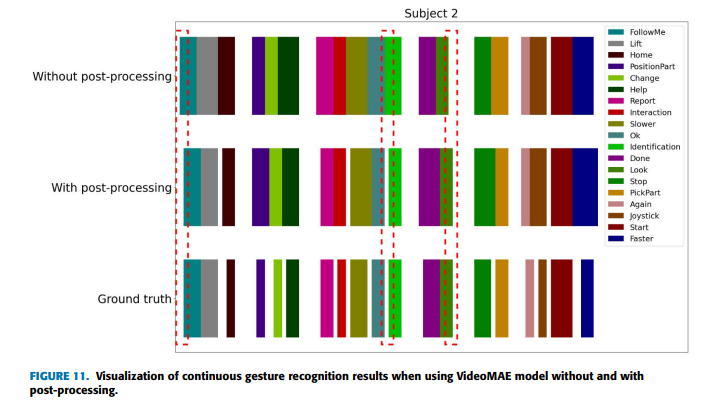
\includegraphics[width=0.94\linewidth]{image-9.png}\par
      \vspace{0.22cm}
      \captiontext{Minh họa kết quả nhận dạng liên tục theo thời gian.}
    \end{column}
  \end{columns}
  \source{Table 6 và Figure 11 trong bài báo}
\end{frame}

\begin{frame}{16. Kết quả trên dataset khác}
  \vspace{0.05cm}
  \begin{columns}[T,onlytextwidth]
    \begin{column}{0.57\textwidth}
      \heading{Đánh giá khả năng tổng quát}
      \begin{itemize}\tightitems
        \item IPN-Hand isolated recognition: \textbf{78.81\% accuracy}.
        \item IPN-Hand continuous recognition: khoảng \textbf{0.80 frame-wise accuracy}, \textbf{0.37 overlap score}.
        \item EgoGesture continuous recognition: khoảng \textbf{0.56 frame-wise accuracy}, \textbf{0.36 overlap score}.
      \end{itemize}
    \end{column}
    \begin{column}{0.39\textwidth}
      \centering
      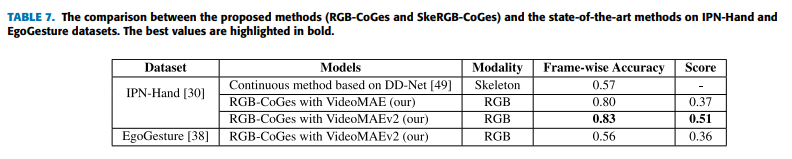
\includegraphics[width=\linewidth]{image-10.png}\par
      \vspace{0.12cm}
      \captiontext{Bảng so sánh kết quả trên IPN-Hand và EgoGesture.}
    \end{column}
  \end{columns}
  \vspace{0.25cm}
  \smallnote{\textbf{Nhận xét:} hiệu năng giảm khi chuyển sang dataset khác do khác biệt về ngữ cảnh, góc nhìn, điều kiện quay và bộ cử chỉ.}
  {\raggedright\source{Table 7 trong bài báo}}
\end{frame}

\begin{frame}{17. Triển khai trên edge device}
  \vspace{0.08cm}
  \begin{columns}[T,onlytextwidth]
    \begin{column}{0.48\textwidth}
      \centering
      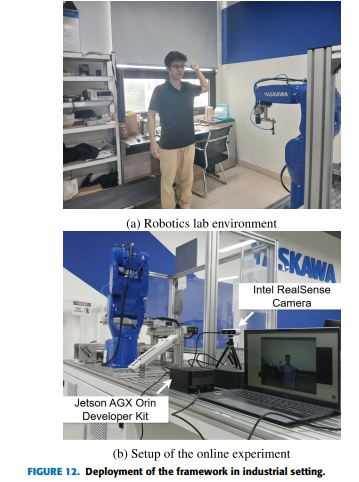
\includegraphics[height=4.55cm]{image-12.png}\par
      \vspace{0.12cm}
      \captiontext{Thiết lập online evaluation trên Jetson AGX Orin.}
    \end{column}
    \begin{column}{0.48\textwidth}
      \heading{Cấu hình thử nghiệm}
      \begin{itemize}\tightitems
        \item Thiết bị: \textbf{Jetson AGX Orin Developer Kit}, GPU, RAM 32GB.
        \item Camera RGB: \textbf{640$\times$480, 30 FPS}.
        \item Skeleton extraction: \textbf{Mediapipe} chạy trên CPU.
        \item Classifier: \textbf{VideoMAE} dùng để phân loại đoạn cử chỉ.
        \item Hệ thống chạy online và đưa ra nhãn dự đoán theo thời gian.
      \end{itemize}
    \end{column}
  \end{columns}
\end{frame}

\begin{frame}{18. Kết quả edge deployment}
  \vspace{0.08cm}
  \begin{columns}[T,onlytextwidth]
    \begin{column}{0.56\textwidth}
      \centering
      {\fontsize{7.8}{9.4}\selectfont
      \renewcommand{\arraystretch}{1.28}
      \begin{tabular}{@{}L{3.68cm}R{1.55cm}@{}}
        \toprule
        \textbf{Chỉ số} & \textbf{Giá trị}\\
        \midrule
        Frame-wise accuracy online & 94\%\\
        Activity overlap score & 56\%\\
        Tốc độ Mediapipe & 4.5 FPS\\
        Tốc độ VideoMAE & 2.5 FPS\\
        Độ trễ trung bình & 1.3 s\\
        Độ trễ đỉnh & trên 2 s\\
        \bottomrule
      \end{tabular}}
    \end{column}
    \begin{column}{0.40\textwidth}
      \heading{Nhận xét}
      \begin{itemize}\tightitems
        \item Accuracy theo frame vẫn cao.
        \item Overlap thấp hơn do lệch biên thời gian.
        \item Tốc độ xử lý thấp hơn camera 30 FPS.
        \item Độ trễ cần giảm trước khi triển khai realtime ổn định.
      \end{itemize}
    \end{column}
  \end{columns}
  \vspace{0.20cm}
  \smallnote{\textbf{Nút thắt:} Mediapipe và VideoMAE xử lý chậm hơn tốc độ ghi hình, gây dropped frames và tăng độ trễ.}
  \source{Table 8 và phần Online Evaluation trong bài báo}
\end{frame}

\begin{frame}{19. Phân tích hạn chế}
  \vspace{0.02cm}
  \heading{Các hạn chế chính}
  \begin{itemize}\tightitems
    \item \textbf{Quy mô dữ liệu:} 50 người và 150 video phù hợp cho nghiên cứu ban đầu, nhưng chưa đại diện đầy đủ cho môi trường công nghiệp rộng.
    \item \textbf{Domain shift:} hiệu năng giảm khi chuyển sang dataset khác do khác biệt góc nhìn, điều kiện quay và bộ cử chỉ.
    \item \textbf{Biên thời gian:} overlap score thấp hơn frame-wise accuracy, cho thấy start/end vẫn là điểm khó.
    \item \textbf{Thiết bị biên:} Mediapipe và VideoMAE xử lý chậm hơn tốc độ camera, gây dropped frames và tăng độ trễ.
  \end{itemize}
  \vspace{0.20cm}
  \begin{tcolorbox}[redbox,title=Nhận định tổng hợp]
    Bài báo đạt kết quả tốt ở năng lực phân loại cử chỉ. Hai hướng cần cải thiện là phân đoạn thời gian và tối ưu tốc độ suy luận trên edge device.
  \end{tcolorbox}
\end{frame}

\begin{frame}{20. Kết luận và hướng phát triển}
  \vspace{0.05cm}
  \begin{columns}[T,onlytextwidth]
    \begin{column}{0.49\textwidth}
      \heading{Kết luận}
      \begin{itemize}\tightitems
        \item CoboGesture bổ sung dataset chuyên biệt cho human-cobot gesture recognition.
        \item RGB-CoGes và SkeRGB-CoGes chuyển bài toán từ isolated sang continuous recognition.
        \item VideoMAE/VideoMAEv2 đạt độ chính xác cao trên isolated recognition.
        \item Edge deployment chứng minh khả năng triển khai, nhưng độ trễ còn lớn.
      \end{itemize}
    \end{column}
    \begin{column}{0.49\textwidth}
      \heading{Hướng phát triển}
      \begin{itemize}\tightitems
        \item Mở rộng dataset về người tham gia, góc nhìn, ánh sáng và môi trường nhà máy thật.
        \item Tối ưu mô hình bằng quantization, TensorRT hoặc kiến trúc nhẹ hơn.
        \item Giảm số frame/độ phân giải đầu vào và xử lý song song các module.
        \item Kết hợp thêm modality khác như giọng nói hoặc tín hiệu an toàn từ robot.
      \end{itemize}
    \end{column}
  \end{columns}
\end{frame}

\end{document}
